\section{Seción} \label{s:section_01}

En este capítulo se muestran varios ejemplos.

\textbf{Negrita} \textit{cursiva}

Hacer una referencia, en este caso al \autoref{s:section_01}.

% ---   ---   --- %


\subsection{Subseccion}

\subsubsection{Citar referencias y acrónimos}

\cite{im78552}, \acrshort{mc}, \acrfull{mc}.

\subsubsection{Enumeraciones}

Enumeración.

\begin{enumerate}
	\item La impresora debe contar con un sistema de nivelación de la base de impresión.
	\item El sistema de extrusión de filamento debe asegurar que no se producirán inconsistencias durante los periodos largos de trabajo.
\end{enumerate}

Enumeración cambiando los items.

\begin{enumerate}[label= \textbf{R-\arabic*}]
	\item La impresora debe contar con un sistema de nivelación de la base de impresión.
	\item El sistema de extrusión de filamento debe asegurar que no se producirán inconsistencias durante los periodos largos de trabajo. \label{req:extrusion}
\end{enumerate}

Referenciar un item: \ref{req:extrusion}, \autoref{req:extrusion}.


Ejemplo de bulletpoints.


\begin{itemize}[label={\scriptsize\raisebox{0.5ex}{\textbullet}}]

	\item Perfilería de aluminio.

\end{itemize}



%   ---   ---   %

\subsubsection{Figuras}

Las figuras se pueden fijar en el texto con H, posicionarlas lo mejor posible con h!, arriba con t, etc.

\begin{figure}[H]
	\centering
	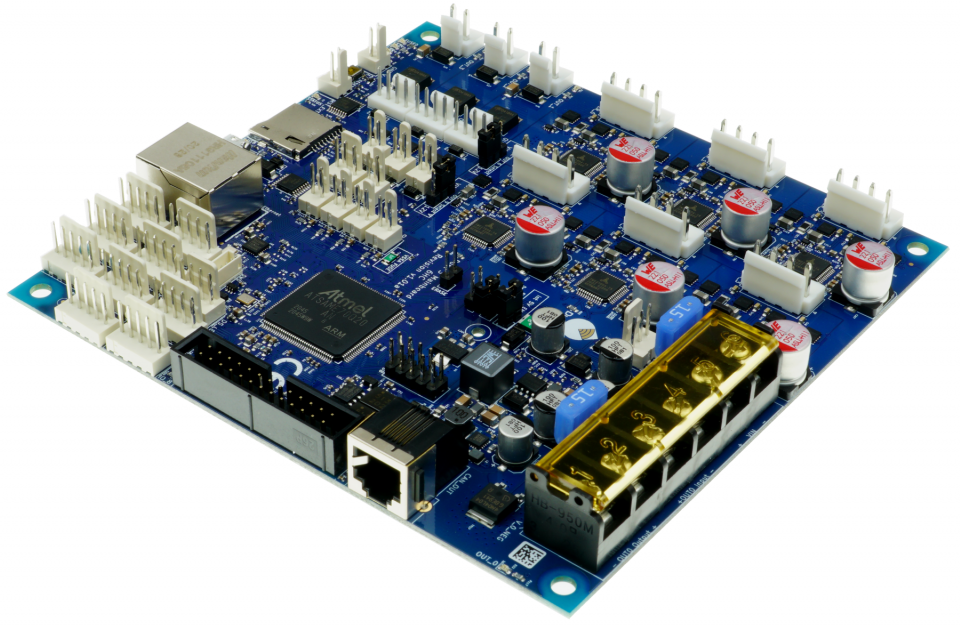
\includegraphics[width=100mm]{duet3}
	\caption{Motherboard Duet 3 6HC.}
	\label{fig:000_00}
\end{figure}

Subfiguras en paralelo.

\begin{figure}[H]
	\centering
	\subfloat[Vista frontal del montaje.\label{fig:mont1}]
	{
		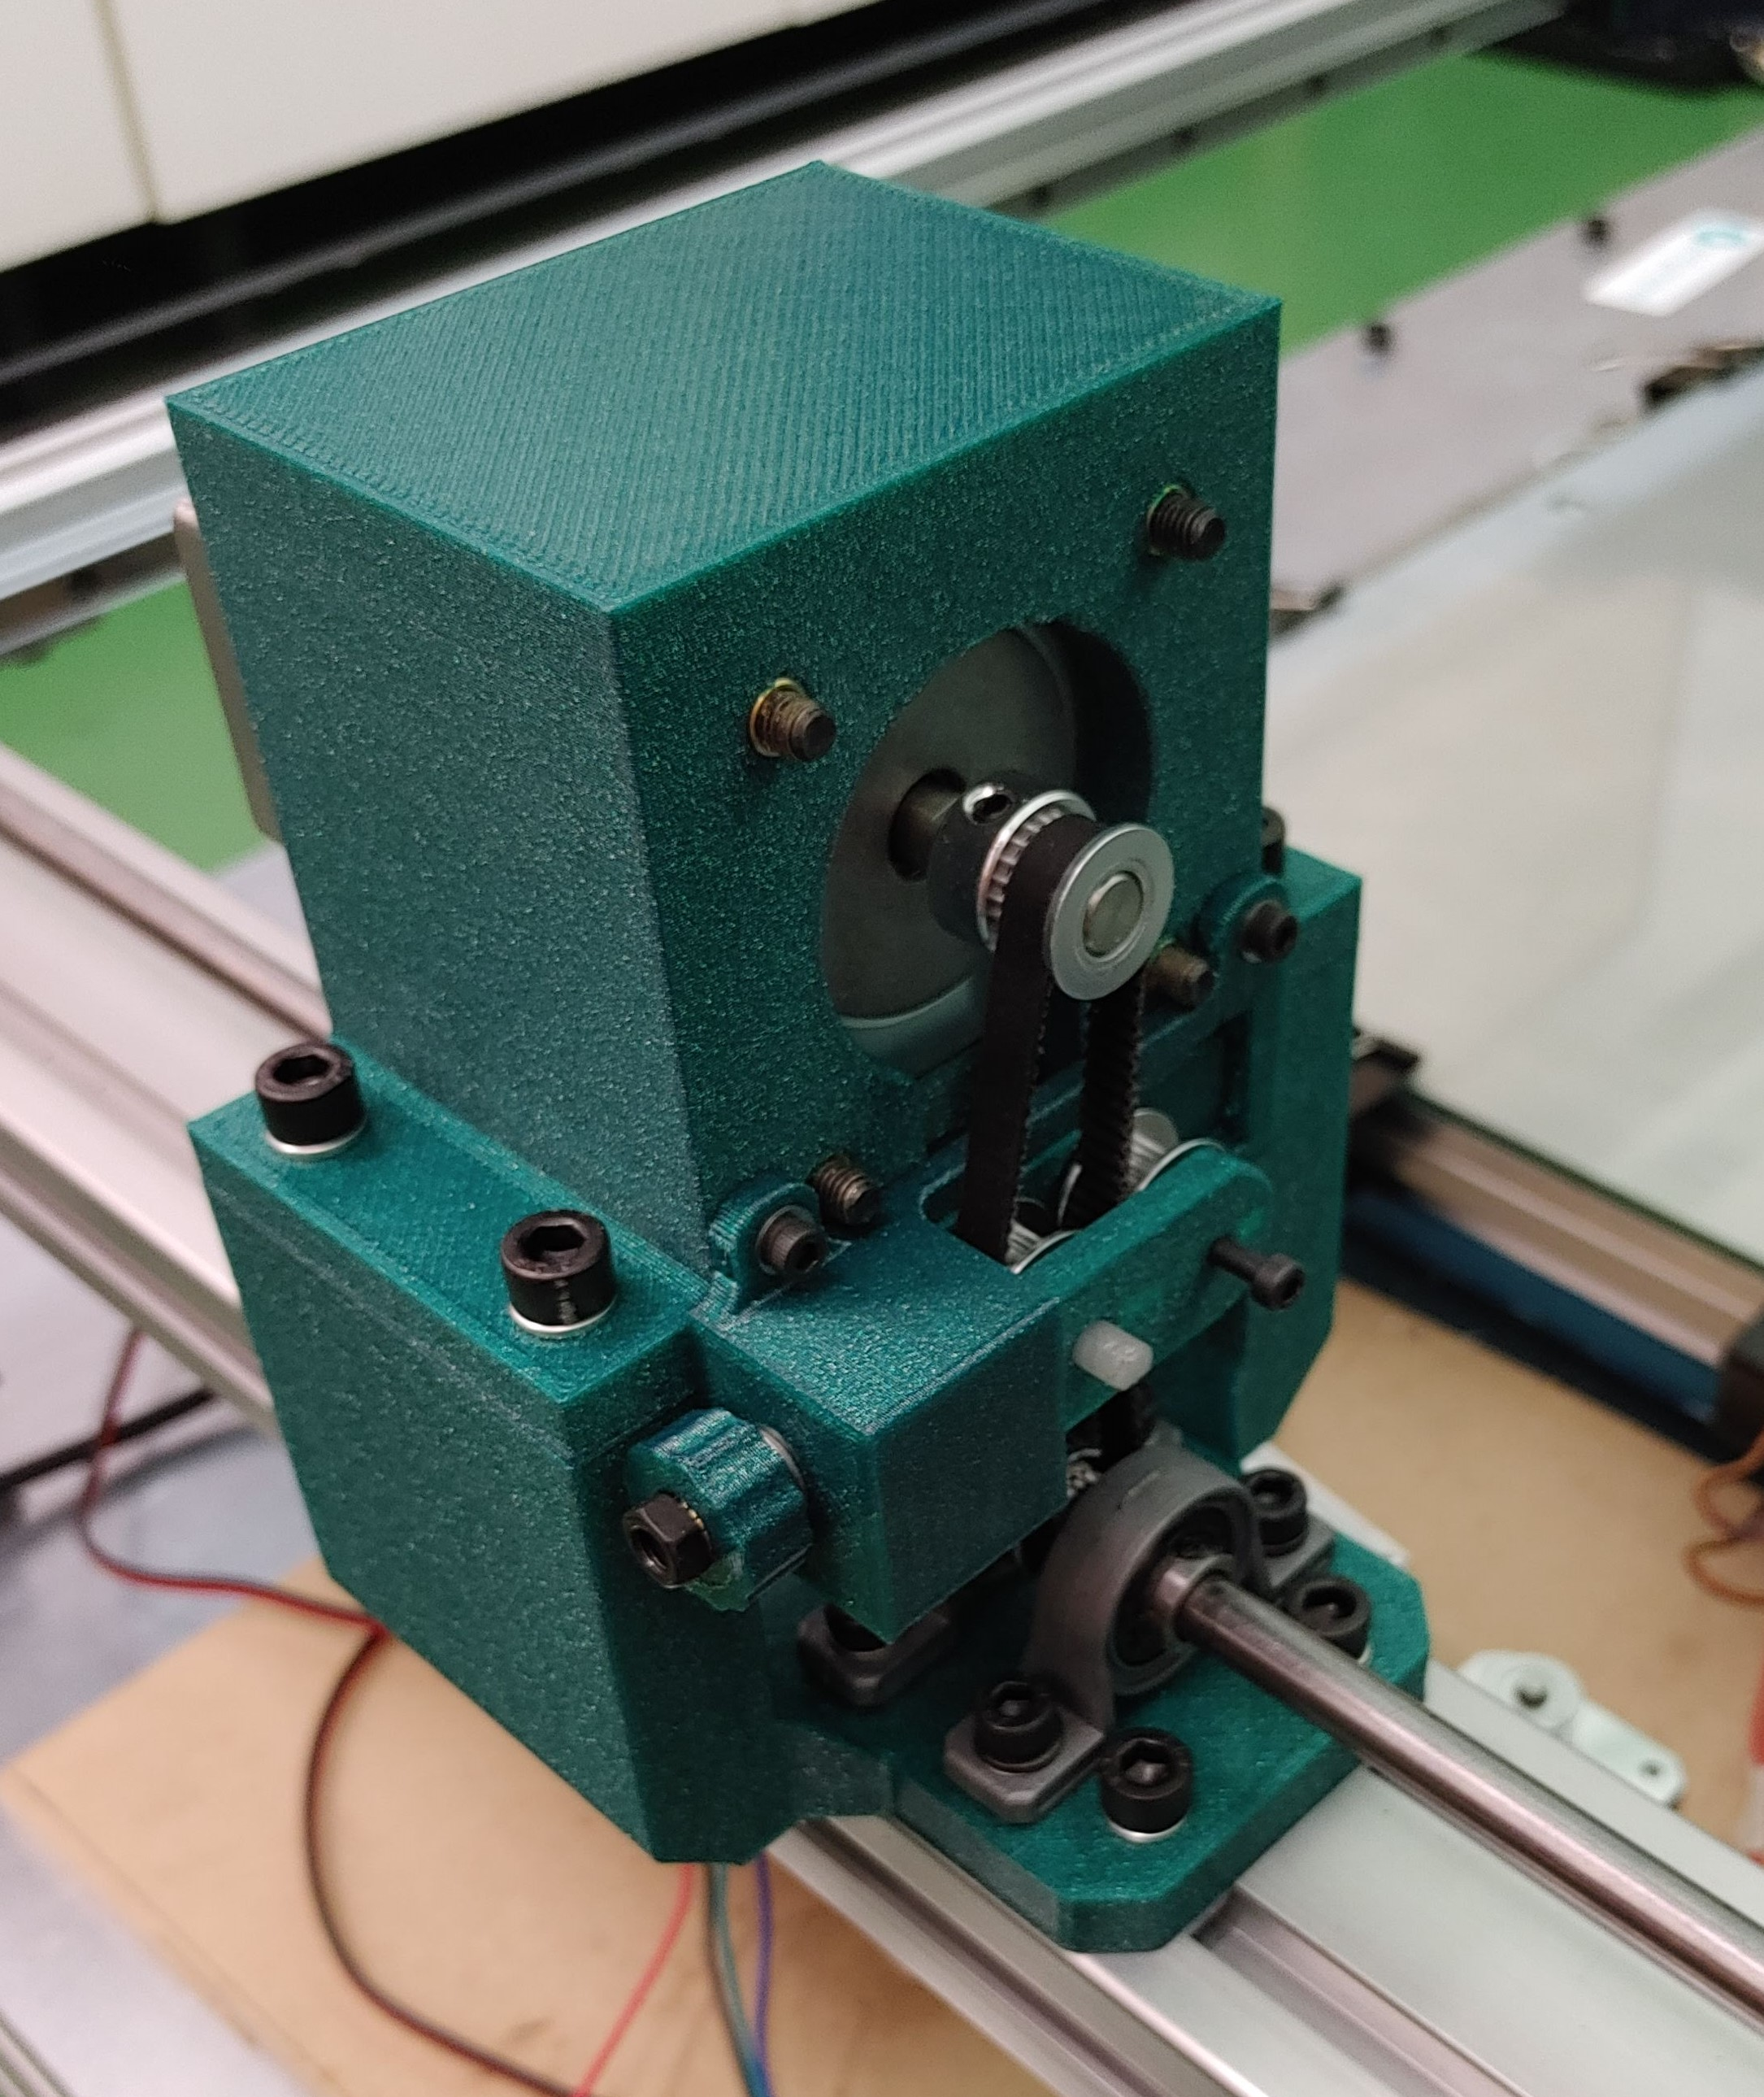
\includegraphics[width=50mm,angle=0]{Mont_01}
	}
	\hspace*{10mm}
	\subfloat[Vista trasera del montaje.\label{fig:mont2}]
	{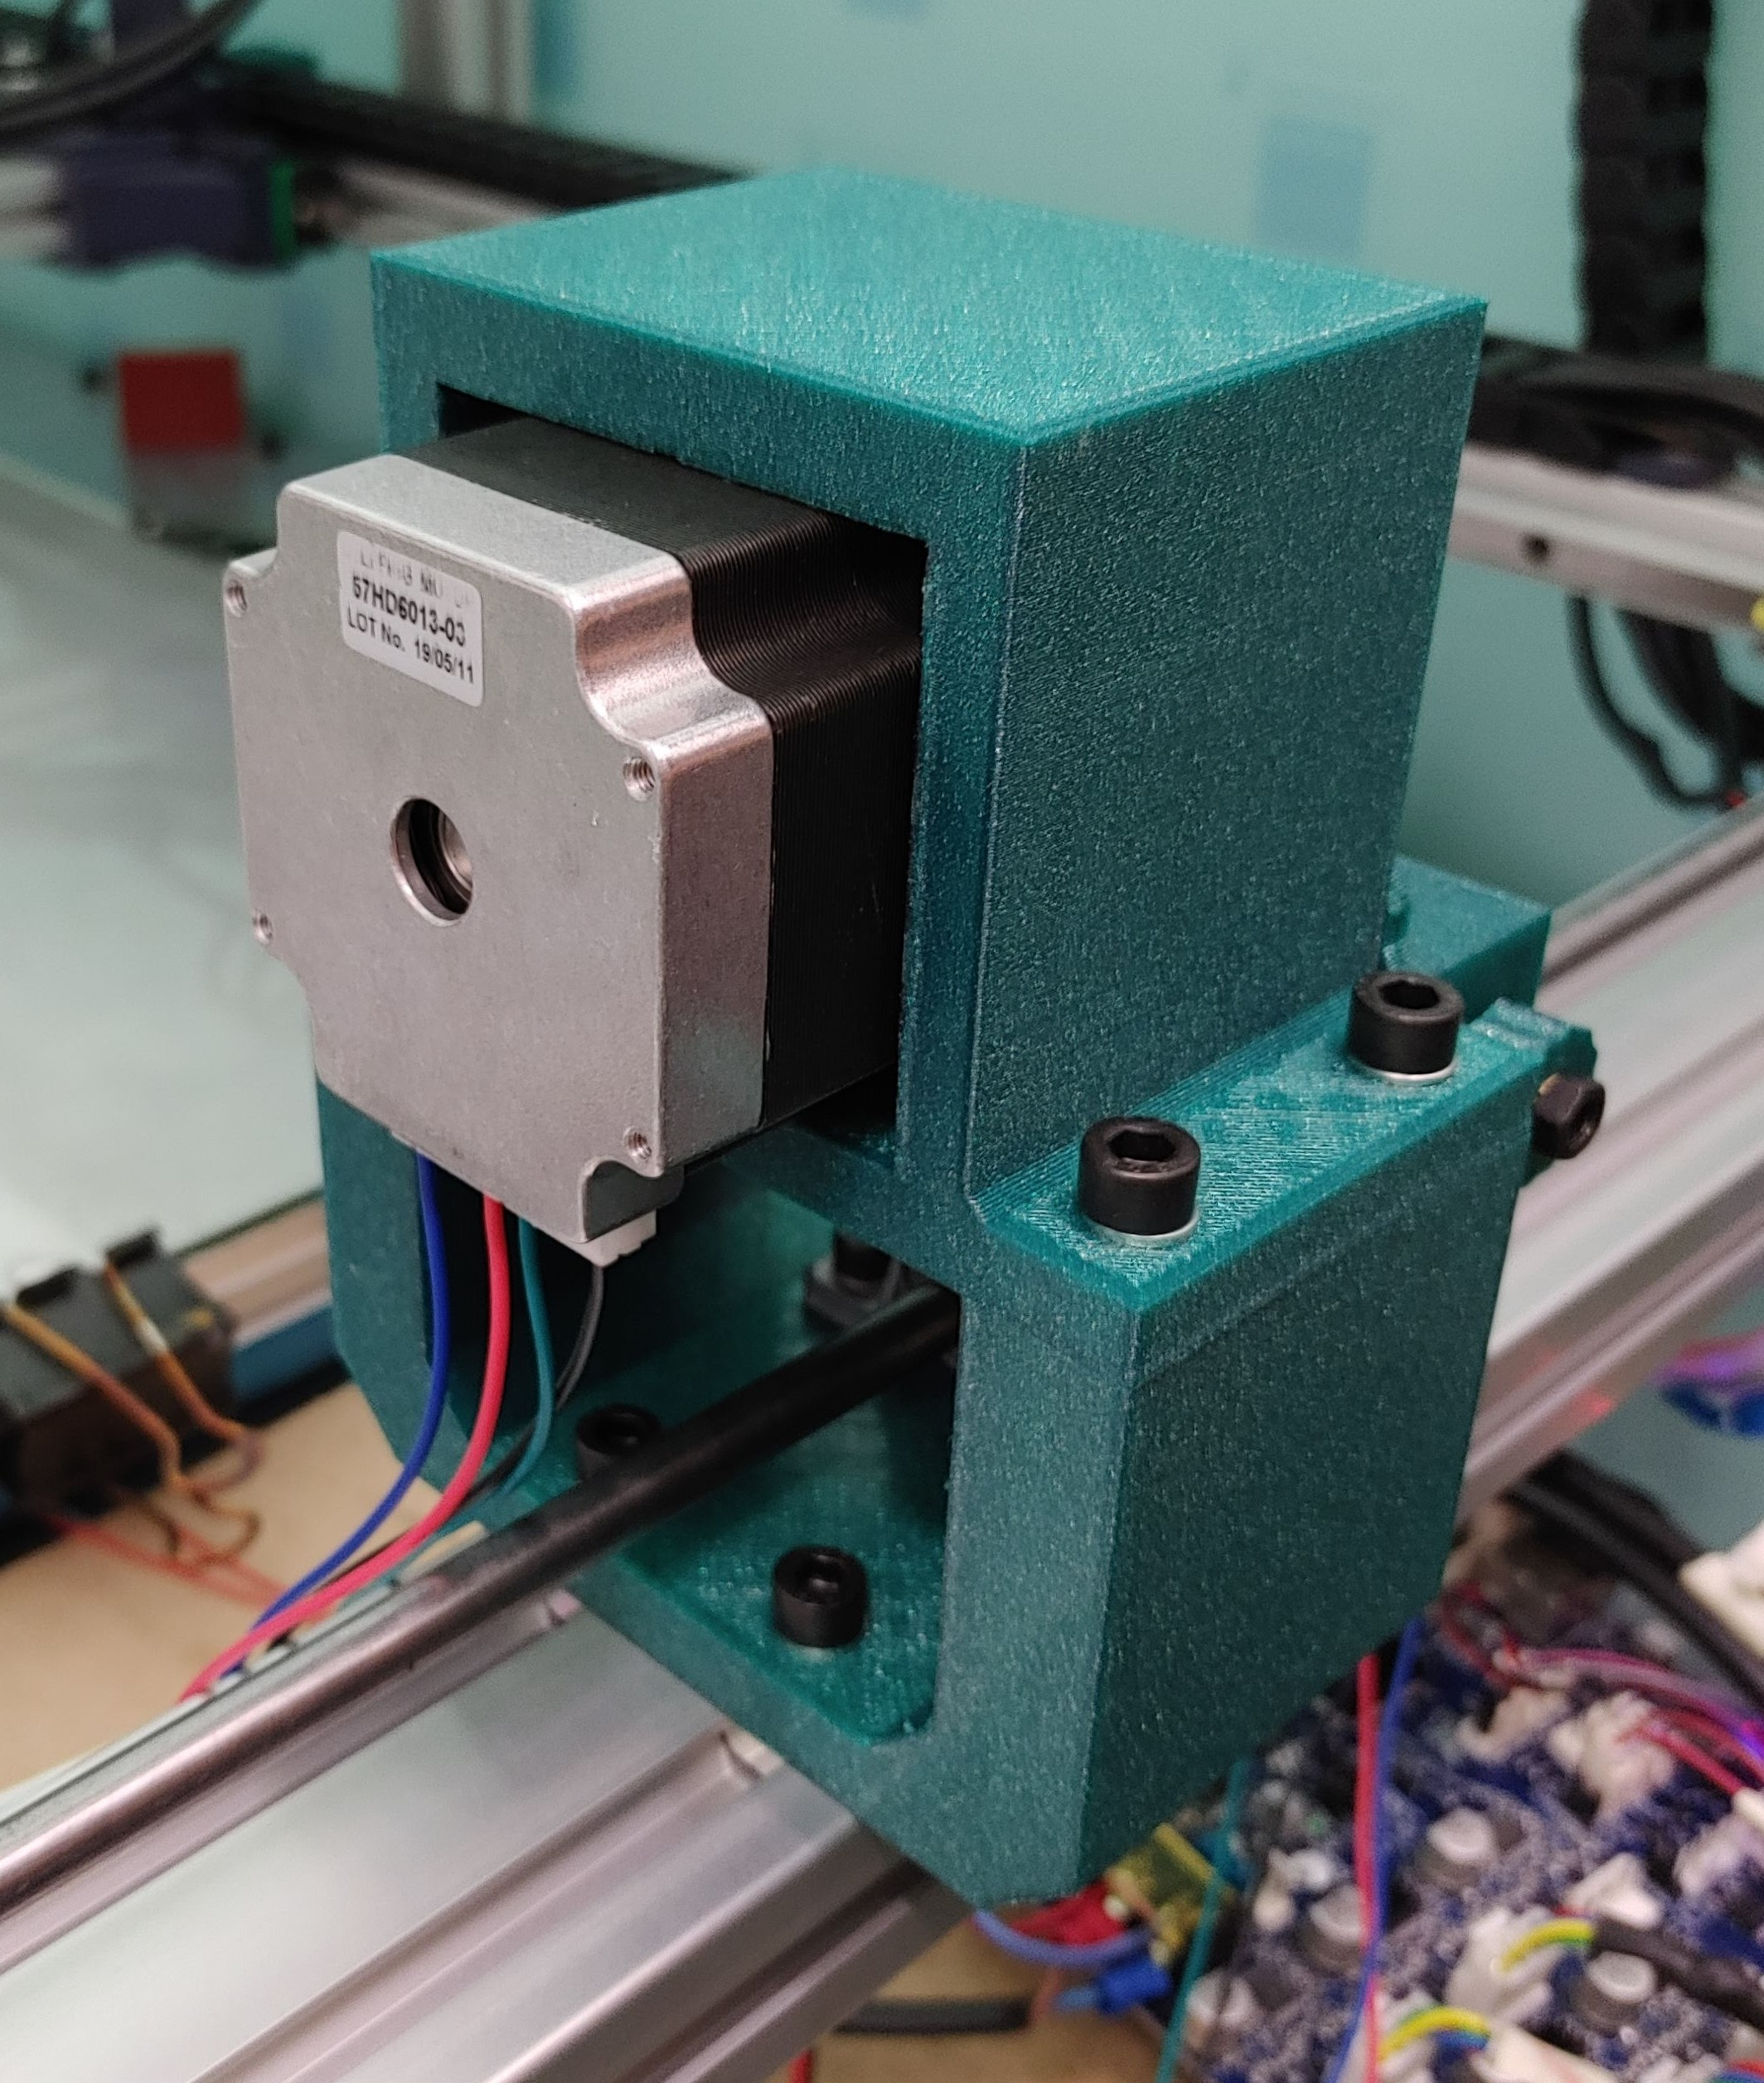
\includegraphics[width=50mm,angle=0]{Mont_02}
	}
	\caption{Montaje del sistema de transmisión del eje X}
	\label{fig:mont_nema}
\end{figure}


Ejemplo dos figuras en paralelo centradas verticalemtne.

\begin{figure}[H]
	\begin{minipage}{\textwidth}
		\centering
		\raisebox{-0.5\height}{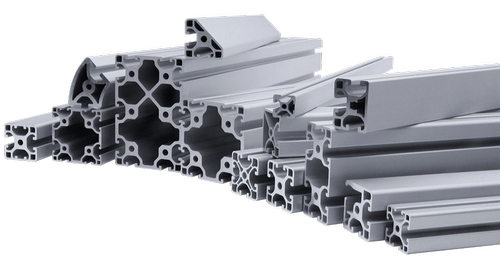
\includegraphics[width=0.4\textwidth]{Perfil_Aluminio}}
	\hspace*{.2in}
		\raisebox{-0.5\height}{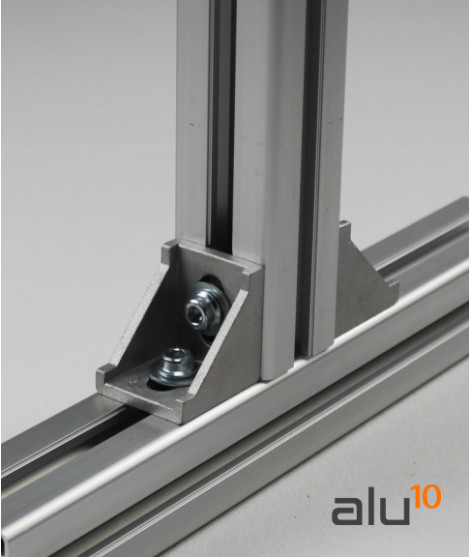
\includegraphics[width=0.25\textwidth]{Perfil_Aluminio_Union}
		}
	\end{minipage}
	\caption{Ejemplos de perfilería de aluminio.}
	\label{fig:perfileria_alumnio}
\end{figure}

Barrera que no pueden atravesar las figuras.
\FloatBarrier


%   ---   ---   %

\subsubsection{Ecuaciones}

Ejemplo de ecuación, \autoref{eq:velocidad}

\begin{equation}\label{eq:velocidad}
	l = \frac{\pi\cdot1.8}{180\cdot P}\cdot r = \frac{\pi\cdot1.8}{180\cdot16}\cdot 6 = 0.0117 \qquad [\mathrm{mm}].
\end{equation}



% ---   ---   --- %

\subsubsection{Tablas}

Ejemplo de tabla de grandes dimensiones e introducir una página apaisada. También se muestra como poner en negrita letras griegas, que a veces dan problemas.

\begin{landscape}
    \vspace*{\fill}
    \begin{table}[H]
    \centering
    \caption{Resultados del estudio paramétrico del modelo de localización (2 de 2).}
        \label{tab:Results_XY_2}
        \resizebox{23cm}{!} {
        {\renewcommand{\arraystretch}{1.2}
        
        
    \begin{tabular}{|r|r|r|r|l|l|l|l|l|l|l|l|l|}
    \hline
    \rowcolor[HTML]{C0C0C0} 
    \multicolumn{1}{|c|}{\cellcolor[HTML]{C0C0C0}} & 
    \multicolumn{3}{c|}{\cellcolor[HTML]{C0C0C0}\textbf{Parámetros}} & 
    \multicolumn{3}{c|}{\cellcolor[HTML]{C0C0C0}\textbf{Distancia}} & 
    \multicolumn{3}{c|}{\cellcolor[HTML]{C0C0C0}\textbf{X}} &
    \multicolumn{3}{c|}{\cellcolor[HTML]{C0C0C0}\textbf{Y}} 
    
    \\ \cline{2-13} 
    
    \rowcolor[HTML]{EFEFEF} 
    \multicolumn{1}{|c|}{\multirow{-2}{*}{\cellcolor[HTML]{C0C0C0}Id}} & 
    \multicolumn{1}{c|}{\cellcolor[HTML]{EFEFEF}\textbf{outFE}} & 
    \multicolumn{1}{c|}{\cellcolor[HTML]{EFEFEF}\textbf{compFE}} & 
    \multicolumn{1}{c|}{\cellcolor[HTML]{EFEFEF}\textbf{compReg}} & 
    \multicolumn{1}{c|}{\cellcolor[HTML]{EFEFEF}$\bm{\mu}$ \textbf{[\%]}} & 
    \multicolumn{1}{c|}{\cellcolor[HTML]{EFEFEF}$\bm{\sigma}$ \textbf{[\%]}} & 
    \multicolumn{1}{c|}{\cellcolor[HTML]{EFEFEF}\textbf{Distribución}} & 
    \multicolumn{1}{c|}{\cellcolor[HTML]{EFEFEF}$\bm{\mu}$ \textbf{[\%]}} & 
    \multicolumn{1}{c|}{\cellcolor[HTML]{EFEFEF}$\bm{\sigma}$ \textbf{[\%]}} & 
    \multicolumn{1}{c|}{\cellcolor[HTML]{EFEFEF}\textbf{Distribución}} & 
    \multicolumn{1}{c|}{\cellcolor[HTML]{EFEFEF}$\bm{\mu}$ \textbf{[\%]}} & 
    \multicolumn{1}{c|}{\cellcolor[HTML]{EFEFEF}$\bm{\sigma}$ \textbf{[\%]}} & 
    \multicolumn{1}{c|}{\cellcolor[HTML]{EFEFEF}\textbf{Distribución}} \\ \hline
    
    25 & 175 & 150 & 100 & \cellcolor[HTML]{606BA3}0.141 & \cellcolor[HTML]{606FA3}0.096 & Generalized Extreme Value & 0.104 & 0.094 & Weibull            & 0.074 & 0.063 & Weibull            \\ \hline
    26 & 175 & 150 & 150 & \cellcolor[HTML]{64B0AC}0.174 & \cellcolor[HTML]{65BBAD}0.124 & Generalized Extreme Value & 0.124 & 0.117 & Exponential        & 0.097 & 0.085 & Weibull            \\ \hline
    27 & 175 & 200 & 100 & \cellcolor[HTML]{617DA5}0.15  & \cellcolor[HTML]{6184A6}0.104 & Generalized Extreme Value & 0.108 & 0.098 & Weibull            & 0.083 & 0.073 & Weibull            \\ \hline
    28 & 175 & 200 & 150 & \cellcolor[HTML]{79C8B0}0.188 & \cellcolor[HTML]{8CD0B1}0.136 & Generalized Extreme Value & 0.131 & 0.126 & Gamma              & 0.108 & 0.097 & Generalized Pareto \\ \hline
    29 & 175 & 250 & 100 & \cellcolor[HTML]{628FA7}0.158 & \cellcolor[HTML]{6292A8}0.109 & Generalized Extreme Value & 0.113 & 0.104 & Weibull            & 0.087 & 0.075 & Weibull            \\ \hline
    30 & 175 & 250 & 150 & \cellcolor[HTML]{9BD6B3}0.2   & \cellcolor[HTML]{BDE4B5}0.149 & Generalized Extreme Value & 0.138 & 0.137 & Gamma              & 0.116 & 0.104 & Weibull            \\ \hline
    31 & 175 & 300 & 100 & \cellcolor[HTML]{6297A9}0.162 & \cellcolor[HTML]{6290A8}0.108 & Generalized Extreme Value & 0.116 & 0.102 & Weibull            & 0.09  & 0.078 & Weibull            \\ \hline
    32 & 175 & 300 & 150 & \cellcolor[HTML]{BBE3B5}0.211 & \cellcolor[HTML]{BBE3B5}0.148 & Generalized Extreme Value & 0.145 & 0.136 & Generalized Pareto & 0.124 & 0.108 & Generalized Pareto \\ \hline
    33 & 200 & 150 & 100 & \cellcolor[HTML]{5E4F9F}0.128 & \cellcolor[HTML]{5E4F9F}0.084 & Generalized Extreme Value & 0.091 & 0.081 & Weibull            & 0.071 & 0.06  & Generalized Pareto \\ \hline
    34 & 200 & 150 & 150 & \cellcolor[HTML]{6290A8}0.159 & \cellcolor[HTML]{628FA7}0.108 & Generalized Extreme Value & 0.113 & 0.101 & Generalized Pareto & 0.089 & 0.077 & Weibull            \\ \hline
    35 & 200 & 200 & 100 & \cellcolor[HTML]{63A7AB}0.17  & \cellcolor[HTML]{63A4AA}0.116 & Generalized Extreme Value & 0.118 & 0.108 & Weibull            & 0.098 & 0.083 & Weibull            \\ \hline
    36 & 200 & 200 & 150 & \cellcolor[HTML]{64B0AC}0.174 & \cellcolor[HTML]{64ABAB}0.118 & Generalized Extreme Value & 0.12  & 0.109 & Generalized Pareto & 0.101 & 0.087 & Weibull            \\ \hline
    37 & 200 & 250 & 100 & \cellcolor[HTML]{617FA5}0.151 & \cellcolor[HTML]{6076A4}0.099 & Generalized Extreme Value & 0.109 & 0.094 & Weibull            & 0.083 & 0.07  & Generalized Pareto \\ \hline
    38 & 200 & 250 & 150 & \cellcolor[HTML]{64B4AC}0.175 & \cellcolor[HTML]{65C0AE}0.126 & Generalized Extreme Value & 0.126 & 0.119 & Gamma              & 0.097 & 0.085 & Weibull            \\ \hline
    39 & 200 & 300 & 100 & \cellcolor[HTML]{6178A4}0.147 & \cellcolor[HTML]{6069A3}0.094 & Gamma                     & 0.105 & 0.091 & Weibull            & 0.082 & 0.068 & Weibull            \\ \hline
    40 & 200 & 300 & 150 & \cellcolor[HTML]{65B9AD}0.178 & \cellcolor[HTML]{6AC2AE}0.127 & Generalized Extreme Value & 0.121 & 0.116 & Gamma              & 0.106 & 0.092 & Weibull            \\ \hline
    41 & 225 & 150 & 100 & \cellcolor[HTML]{628BA7}0.156 & \cellcolor[HTML]{628FA7}0.107 & Generalized Extreme Value & 0.115 & 0.104 & Weibull            & 0.083 & 0.071 & Weibull            \\ \hline
    42 & 225 & 150 & 150 & \cellcolor[HTML]{5F66A2}0.139 & \cellcolor[HTML]{6072A4}0.097 & Generalized Extreme Value & 0.1   & 0.091 & Weibull            & 0.077 & 0.066 & Weibull            \\ \hline
    43 & 225 & 200 & 100 & \cellcolor[HTML]{639EAA}0.166 & \cellcolor[HTML]{6292A8}0.109 & Generalized Extreme Value & 0.12  & 0.105 & Generalized Pareto & 0.09  & 0.076 & Weibull            \\ \hline
    44 & 225 & 200 & 150 & \cellcolor[HTML]{6296A8}0.161 & \cellcolor[HTML]{63A6AA}0.116 & Generalized Extreme Value & 0.113 & 0.109 & Gamma              & 0.093 & 0.079 & Weibull            \\ \hline
    45 & 225 & 250 & 100 & \cellcolor[HTML]{606FA3}0.143 & \cellcolor[HTML]{6069A3}0.094 & Generalized Extreme Value & 0.1   & 0.089 & Weibull            & 0.082 & 0.068 & Weibull            \\ \hline
    46 & 225 & 250 & 150 & \cellcolor[HTML]{6296A8}0.161 & \cellcolor[HTML]{6399A9}0.112 & Generalized Extreme Value & 0.115 & 0.107 & Gamma              & 0.09  & 0.075 & Weibull            \\ \hline
    47 & 225 & 300 & 100 & \cellcolor[HTML]{6184A6}0.153 & \cellcolor[HTML]{6186A6}0.104 & Generalized Extreme Value & 0.114 & 0.103 & Weibull            & 0.08  & 0.066 & Weibull            \\ \hline 
    \end{tabular}
    
        }
        }
    \end{table}
    \vspace*{\fill}
    \clearpage
\end{landscape}


% ---   ---   --- %

\subsubsection{Código}


\begin{lstlisting}
M303 H0 S60 ; auto tune heater 0, default PWM (100%), 60C target
M303        ; report the auto-tune status or last resulM303 ; report the auto-tune status or last result
M500        ; save parameters
\end{lstlisting}

\lstinputlisting{Code/function.m}


